% Created 2013-09-10 Tue 22:06
\documentclass[11pt]{article}
\usepackage[utf8]{inputenc}
\usepackage[T1]{fontenc}
\usepackage{graphicx}
\usepackage{longtable}
\usepackage{float}
\usepackage{wrapfig}
\usepackage{soul}
\usepackage{amssymb}
\usepackage{hyperref}
\usepackage{svn}
\usepackage[T1]{fontenc}
\usepackage{mathpazo}
\usepackage[margin=1.3in]{geometry}
\linespread{1.05}
\usepackage[scaled]{helvet}
\usepackage{courier}
\usepackage{varioref}
\usepackage[usenames,dvipsnames]{color}
\usepackage{hyperref}
\hypersetup{colorlinks=true,linkcolor=blue,urlcolor=RawSienna}
\floatplacement{figure}{H}
\floatplacement{table}{H}
\newcommand{\hilight}[1]{\colorbox{yellow}{#1}}

\title{Solution Architecture Definition for ``Mirroring of Virtual-labs at IITD''}
\author{Suraj Samal}
\date{10 September 2013}

\begin{document}

\maketitle

\setcounter{tocdepth}{3}
\tableofcontents
\vspace*{1cm}

\listoftables
\listoffigures

\section{DOCUMENT NAME AND STATUS}
\label{sec-1}




\begin{center}
\begin{tabular}{l}
\hline
 Solution Architecture Definition  \\
\hline
\end{tabular}
\end{center}




\begin{center}
\begin{tabular}{l}
\hline
 \textbf{Mirroring of Virtual-labs at IITD}  \\
 \emph{Lab Sources and VLEAD VMs}            \\
\hline
\end{tabular}
\end{center}




\begin{center}
\begin{tabular}{lr}
\hline
 Document Status:  &       Draft  \\
 Document Issue:   &         0.2  \\
 Issue date:       &  2013-09-06  \\
\hline
\end{tabular}
\end{center}


                                      
\section{DOCUMENT PURPOSE}
\label{sec-2}

The Solution Architecture Definition defines the overall
architectural solution for the ``Mirroring of Virtual-labs at
IITD''. The solution addresses the problem as documented in the ``VLEAD
Mandate - Virtual Labs Integration: Deliverables, Resources and Budget
2012-06-02''.  The solution comprises a number of elements
or components, which are partitioned into subsets for
implementation. The primary audience of this document consists of IT
and network architects.The primary purpose of this document is to
communicate the essential elements of the overall solution so that
operatational implications can be assessed and understood, and so that
the design activities in Design \& Build can proceed further.  
As such it tries to achieve the following:
\begin{itemize}
\item It provides visibility and exposure to other architects for peer
  review.
\item It unambiguously defines the overall solution to the proposed
  requirements of the initiative.
\item It provides a basis for assessment of the overall solution once
  implemented.
\item It describes how the development and deployment of the solution can
  be phased if this is required to meet needs and or to meet
  technology constraints
\end{itemize}
\section{PROJECT OVERVIEW AND STATUS}
\label{sec-3}


VLEAD (Virtual Labs Engineering and Architecture Division) team was
setup in June 2012 as a central engineering team for integrating all
the virtual-labs (around 180 in number) across all disciplines and
institutes onto a common data-center (currently located at IIIT
Hyderabad). Currently(as of 2013-08-15) around 86 lab sources are
version-controlled and around 40 hosted out of IIIT
data-centre. Hence, it becomes absolutely necessary to have atleast
the sources mirrored at an additional location (identified as IIT
Delhi) so as to ensure availability, reliability and faster recovery
of \textbf{Virtual Labs} in case of unforeseen disasters or catastropes.

In very long term, the plan is to achieve live mirroring of all the
  lab content as well as to run \textbf{Virtual labs} out of multiple sites
  to ensure better availability, reliability and performance.

\section{PROJECT SCOPE}
\label{sec-4}


 The scope of this project is to have the sources of all the
Virtual-labs mirrored at one of the servers at IIT
Delhi. Additionally, other critical data on VLEAD VMs and containers
are also planned to be mirrored as part of this initiative.


\begin{table}[H]
\caption{\label{tbl:Inclusions and Exclusions}Project Scope - Inclusions and Exclusions}
\begin{center}
\begin{tabular}{ll}
\hline
 Inclusions             &  Exclusions                            \\
\hline
 Backup of Lab Sources  &  Live Mirroring of lab                 \\
                        &  content and hosting                   \\
 Backup of VMs and      &  Mirroring of complete VLEAD Services  \\
 Containers             &  Load-sharing between IIITH            \\
                        &  and IITD sites                        \\
\hline
\end{tabular}
\end{center}
\end{table}

\section{PROJECT ROLES AND RESPONSIBILITIES}
\label{sec-5}

\subsection{Key Stakeholders}
\label{sec-5.1}



\begin{table}[H]
\caption{\label{tbl:Key Stakeholders}Key Stakeholders}
\begin{center}
\begin{tabular}{lll}
\hline
 AREA / POSITION  &  NAME                 &  ROLE                  \\
\hline
 Prime            &  Ranjan Bose          &  Virtual-labs Project  \\
 Stakeholders     &                       &  Co-Investigator       \\
                  &                       &  (IIT Delhi)           \\
                  &  Venkatesh Choppella  &  VLEAD Project Head    \\
                  &                       &  (IIIT Hyderabad)      \\
\hline
 Technology       &  Chandan Gupta        &  Technical Manager     \\
 Stakeholders     &                       &  (IIIT Hyderabad)      \\
 (IT, Vendors,    &  Kuldeep Singh        &  Project Associate     \\
 Networks etc)    &                       &  (IIT Delhi)           \\
                  &  Suraj Ketan Samal    &  Engineer              \\
                  &                       &  (IIIT Hyderabad)      \\
                  &  Tech Support Group   &  Technical Support     \\
                  &                       &  (IIIT Hyderabad)      \\
\hline
\end{tabular}
\end{center}
\end{table}

\subsection{Escalation Levels}
\label{sec-5.2}



\begin{table}[H]
\caption{\label{tbl: Escalation Levels}Escalation Levels}
\begin{center}
\begin{tabular}{lllr}
\hline
 Escalation Level  &  NAME                 &  Email                           &   CONTACT NUMBER  \\
\hline
 LEVEL 3           &  Ranjan Bose          &  rbose.iitd@gmail.com            &  +91-11-26591048  \\
                   &  (IIT Delhi)          &                                  &                   \\
 LEVEL 3           &  Venkatesh Choppella  &  venkatesh.choppella@iiit.ac.in  &  +91-965-2740281  \\
                   &  (IIIT Hyderabad)     &                                  &                   \\
\hline
 LEVEL 2           &  Chandan Gupta        &  chandan@virtual-labs.ac.in      &  +91-970-3330781  \\
                   &  (IIIT Hyderabad)     &                                  &                   \\
 LEVEL 2           &  Kuldeep Singh        &  kuldeep.002@gmail.com           &  +91-11-64674687  \\
                   &  (IIT Delhi)          &                                  &                   \\
\hline
 LEVEL 1           &  Suraj Ketan Samal    &  suraj@virtual-labs.ac.in        &  +91-868-6160862  \\
                   &  (IIIT Hyderabad)     &                                  &                   \\
 LEVEL 1           &  <To be Added>        &  <To be Added>                   &    <To be Added>  \\
                   &  (IIT Delhi)          &                                  &                   \\
\hline
 LEVEL 0           &  Technical Support    &  engg@virtual-labs.ac.in         &  +91-40-66531592  \\
                   &  (IIIT Hyderabad)     &                                  &                   \\
\hline
\end{tabular}
\end{center}
\end{table}


\subsection{Escalation Matrix}
\label{sec-5.3}


 Below is the proposed response-time for various types of requests:


\begin{table}[H]
\caption{\label{tbl: Escalation Matrix}Escalation Matrix}
\begin{center}
\begin{tabular}{lll}
\hline
 Escalation Level/Request Type  &  Urgent  &  Normal   \\
\hline
 LEVEL 0                        &  2 hrs   &  2 days   \\
 LEVEL 1                        &  4 hrs   &  5 days   \\
 LEVEL 2                        &  6 hrs   &  10 days  \\
 LEVEL 3                        &  1 day   &  15 days  \\
 LEVEL 4                        &  3 days  &  25 days  \\
\hline
\end{tabular}
\end{center}
\end{table}


Note: 
\begin{itemize}
\item `hrs' mean working hours and `day' or `days' mean working days
\item `response-time' means acknowledgement of the issue and work in progress on the same
\end{itemize}
 
\begin{itemize}
\item Below is the description of various Request Types:
\end{itemize}
\begin{table}[H]
\caption{\label{tbl:Request Types}Request Types}
\begin{center}
\begin{tabular}{ll}
\hline
 Request Type  &  Description                                             \\
\hline
 Urgent        &  The complete solution or majority of the solution       \\
               &  is affected. (Ex: Backups not happening any more due    \\
               &  to some bug in the solution, Network Issues due to ISP  \\
               &  down, power outage etc)                                 \\
 Normal        &  Minor bugs with little impact on the solution,          \\
               &  change requests to the existing solution,               \\
               &  and maintainance activities                             \\
\hline
\end{tabular}
\end{center}
\end{table}


\section{SOLUTION ARCHITECTURE ASSUMPTIONS}
\label{sec-6}



\begin{table}[H]
\caption{\label{tbl:Assumptions}Solution Architecture Assumptions}
\begin{center}
\begin{tabular}{lll}
\hline
 Table 1.  &  Assumptions     &                                                    \\
\hline
 Number    &  Assumption      &  Description                                       \\
\hline
 ASS-01    &  Resources       &  Resources should be available at                  \\
           &                  &  (IIITH and IITD) for setup and continuous         \\
           &                  &  support (trouble-shooting, fixing issues)         \\
           &                  &  throughout the duration of Virtual-Labs project   \\
 ASS-02    &  Infrastructure  &  Infrastructure at IIT Delhi will need to be       \\
           &                  &  setup within appropiate time-frames. It           \\
           &                  &  should be accessible from Virtual-labs            \\
           &                  &  datacenter,IIIT Hyderabad.                        \\
 ASS-03    &  Data            &  Data content and format for the mirroring-setup   \\
           &  requirements    &  will not vary without agreement between VLEAD,    \\
           &                  &  IIIT Hyderabad and Virtual-labs,IIT Delhi teams.  \\
 ASS-04    &  Estimated       &  Labs Assumed =180, VMs Assumed = 55, Also,        \\
           &  Data            &  it doesnot include backups of individual VMs      \\
           &                  &  (one-vm-per lab model).                           \\
 ASS-05    &  Change          &  All subsequent changes to this interface will     \\
           &  management      &  need to be signed off by all the prime            \\
           &                  &  Stakeholders and updated accordingly in           \\
           &                  &  this document.                                    \\
\hline
\end{tabular}
\end{center}
\end{table}


\section{SOLUTION OVERVIEW}
\label{sec-7}

\subsection{Current Architecture Overview}
\label{sec-7.1}


\begin{figure}[H]
\centering
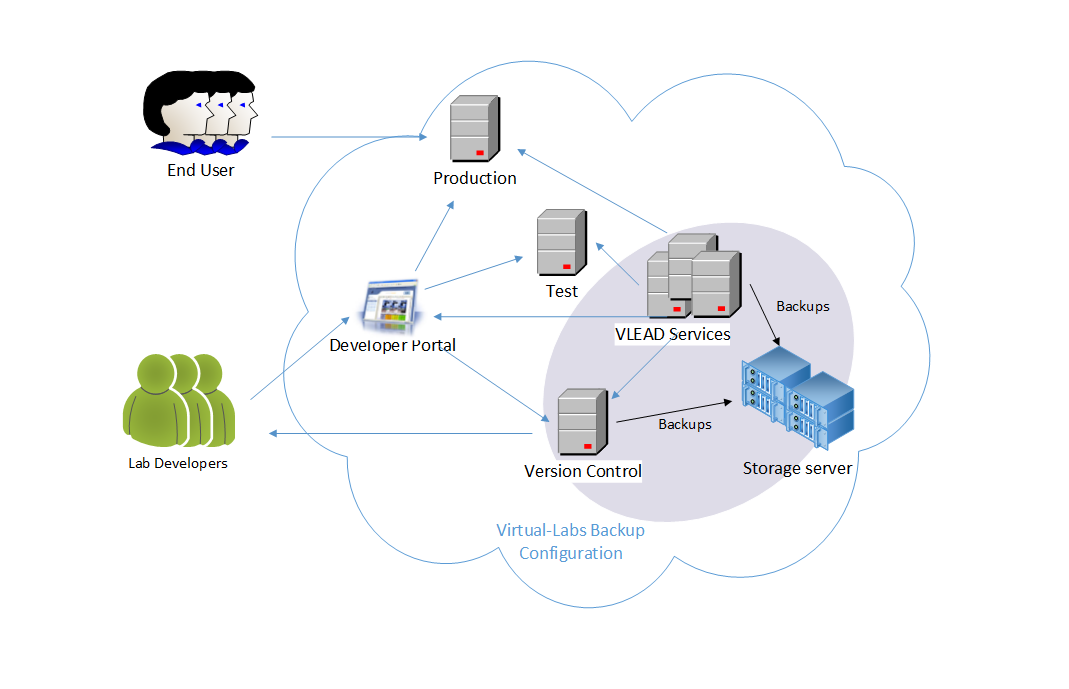
\includegraphics[width=16cm]{Current-Backup-Model.png}
\caption{Current Architecture}
\end{figure}

    Sources of all virtual-labs are stored in the version-control
VM(\emph{svn.virtual-labs.ac.in/bzr.virtual-labs.ac.in/git.virtual-labs.ac.in})
at Virtual Labs DataCenter, IIIT Hyderabad. These sources are uploaded
(checked-in) and downloaded (checked-out) over HTTP and SSH publicly
by different lab developers across all the institutes. This critical
data is already backed-up on a storage server(SAN) located in the same
data-center.
  
  Additionally, there is also critical data belonging to services
provided by VLEAD (\emph{eg. ldap, developer-portal, ns, mail}) which is used
by Virtual-labs community and VLEAD internally. This data is across
different Virtual machines setup at Virtual Labs DataCenter, IIIT
Hyderabad. Selected file-systems from all these VMs is already
backed-up on the same storage server(SAN) in the existing data-center.
\subsection{Proposed Architecture Overview}
\label{sec-7.2}


   \begin{figure}[H]
\centering
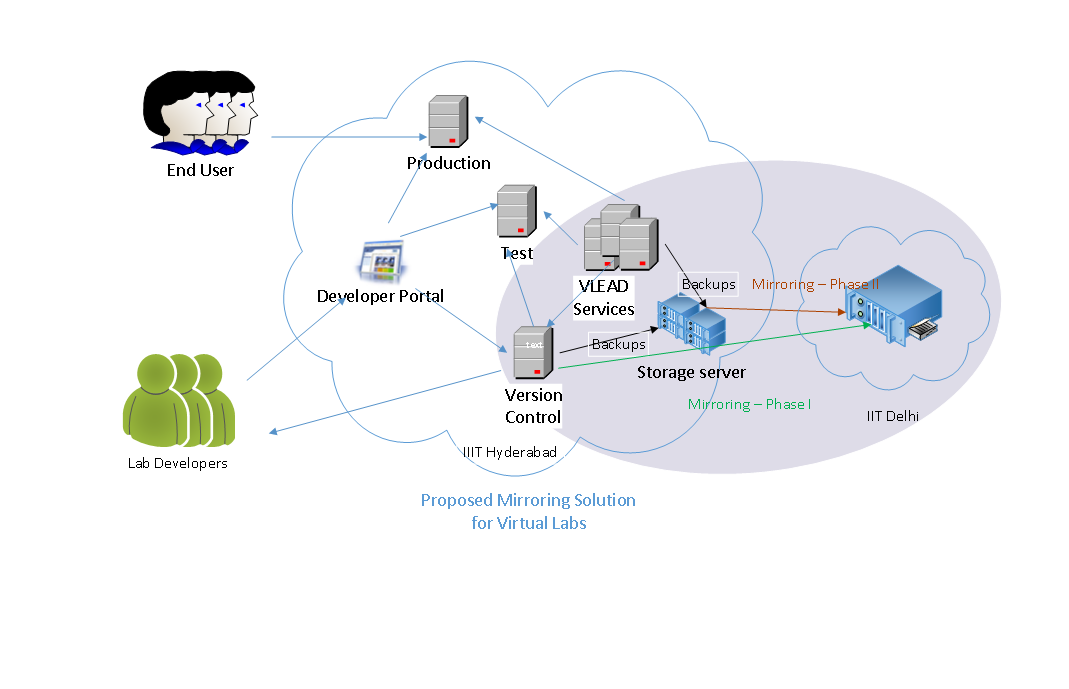
\includegraphics[width=16cm]{./Mirroring-Proposed.png}
\caption{Proposed Architecture}
\end{figure}

\begin{itemize}
\item All the critical data(as described above) at IIIT DataCenter
   will be mirrored at an offsite location(IIT, Delhi) using a
   mechanism that syncs data overnight at a specified time everyday.
\item In Phase-I, a overnight cronjob would be scheduled at the IIIT
   data-center to push all the virtual-lab sources from
   version-control server to the mirrored location at IITD.
\item In Phase-II, the cronjob would be modified to additionally backup
   VLEAD service VMs from the storage server(SAN) to mirrored location at IITD.
\end{itemize}
\subsection{Architectural Decisions}
\label{sec-7.3}

     Here are a summary of significant decisions and the rationale behind
the decisions used to derive the solution. This table represents a
single decision and each decision in a table format.


\begin{table}[H]
\caption{\label{tbl:Backup Principle}Architectural Decisions}
\begin{center}
\begin{tabular}{ll}
\hline
 Subject Area            &  Area of Concern                                                            \\
\hline
 Architectural Desicion  &  AD-001 Backup principle                                                    \\
 Issue or Problem        &  Which backup/restore tool should be used ?                                 \\
 Assumptions             &                                                                             \\
 Motivation              &  - Data sizes are huge, hence need to have a mechanism to                   \\
                         &  send incremental data rather than sending all the data everytime.          \\
                         &  - Backup/Restore process should be recoverable, so that                    \\
                         &  in case of failure, it can start from the place it failed.                 \\
                         &  - Backup/Restore process should work seamlessly with a subset              \\
                         &  of data without any additional efforts.                                    \\
                         &  - Transfer of data over public network should be secure and encrypted.     \\
                         &  - Should be scalable (atleast up to the estimated specifications).         \\
                         &  - Should complete within stipulated time-frames and not interfere          \\
                         &  with system's normal operations.                                           \\
                         &  - Should be automated requiring as less manual intervention as possible.   \\
                         &  - Backup tool should preserve the user/group/timestamp attributes.         \\
                         &  - Data needs to be pushed rather than pulled to enable VLEAD               \\
                         &  team to monitor the backup/restore process.                                \\
                         &  - Should send data with parallel/simultaneous connections and              \\
                         &  in compressed format.                                                      \\
 Options                 &  Rsync, SCP (Secure Copy), Rsnapshot(uses rsync),                           \\
                         &  Clonezilla (works at image level)                                          \\
 Decision                &  `rsync' tool to be used and scheduled on crontab. Data will be pushed      \\
                         &  from the source to the destination.                                        \\
 Justification           &  Rsync seems to closely satisfy all the requirements as mentioned earlier:  \\
                         &  - SCP cant be used in an incremental fashion and doesnot preserve          \\
                         &  filesystem attributes.                                                     \\
                         &  - Rsnapshot is a good tool but applicable when it runs on destination and  \\
                         &  pulls data from source.                                                    \\
                         &  - Clonezilla or other Imaging tools work at disk/filesystem level and      \\
                         &  not applicable in complete or partial backup/restore of directories.       \\
 Implications            &  `rsync' tool should be available on both the systems and an SSH account    \\
                         &  on the mirror-system is required                                           \\
 Derived requirements    &  Rsync should be installed on both source and destination systems.          \\
 Related Decisions       &                                                                             \\
\hline
\end{tabular}
\end{center}
\end{table}



\begin{table}[H]
\caption{\label{tbl:Platform Specifications}Architectural Decisions}
\begin{center}
\begin{tabular}{ll}
\hline
 Subject Area            &  Area of Concern                                                           \\
\hline
 Architectural Decision  &  AD-002 Mirrored Platform Specifications                                   \\
 Issue or Problem        &  Which hardware/OS/softwares should be used for the target mirror          \\
                         &  destination and what should be its specifications ?                       \\
 Assumptions             &                                                                            \\
 Motivation              &  - Existing lab sources are versioned on linux platforms(open source).     \\
                         &  Hence mirrored location should also be Linux based                        \\
                         &  so as to make the backup/restore process simpler.                         \\
                         &  - Destination platform should be reliable, available and provide          \\
                         &  optimum performance.                                                      \\
                         &  - Mirrored location should be operational remotely (aleast from           \\
                         &  IIIT Hyderabad).                                                          \\
                         &  - Server should be accessible from Virtual-labs network, IIIT Hyderabad.  \\
 Options                 &                                                                            \\
 Decision                &  - Standard Platform (Multi-core Intel Xeon Series Processor)              \\
                         &  - Atleast 16GB of RAM                                                     \\
                         &  - Atleast 1TB of available space after (RAID)                             \\
                         &  - Redundant power backup                                                  \\
                         &  - RAID Configured for reliability and optimum performance.                \\
                         &  - Multiple network interfaces (if possible).                              \\
                         &  - An SSH account is required for maintainance purposes.                   \\
                         &  - Rsync tool is required and should run on a port accessible              \\
                         &  form Virtual-labs network.                                                \\
 Justification           &  Decisions made according to items required in the Motivation section      \\
 Implications            &                                                                            \\
 Derived requirements    &                                                                            \\
 Related Decisions       &                                                                            \\
\hline
\end{tabular}
\end{center}
\end{table}


\subsection{Architectural Issues}
\label{sec-7.4}



\begin{table}[H]
\caption{\label{tbl:Architectural Issues}Key Architectural Issues}
\begin{center}
\begin{tabular}{llll}
\hline
 Issue       &  Area(s)      &  Description                              &  Status  \\
 Identifier  &  Impacted     &                                           &          \\
\hline
 ISS – 01    &  Backup Data  &  Version control is currently             &  Closed  \\
             &               &  in a different network                   &          \\
             &               &  (10.4.7.x) and needs to be               &          \\
             &               &  migrated to (10.4.12.x) network          &          \\
             &               &  before the solution is implemented.      &          \\
 ISS - 02    &  Security     &  Data on mirrored-location can be         &  Open    \\
             &               &  accessible to anyone having physical     &          \\
             &               &  access to the system as it is a          &          \\
             &               &  file-system backup.                      &          \\
 ISS - 03    &  Backup Tool  &  Rsync has problem with higher            &  Open    \\
             &               &  file-sizes (>2GB)                        &          \\
 ISS - 04    &  Network      &  Overall link bandwidth might not be      &  Open    \\
             &  Bandwidth    &  reliable and intermittently slow.        &          \\
             &               &  We should probably investigate use of a  &          \\
             &               &  dedicated service line from IIIT         &          \\
             &               &  Hyderabad to IITD based on the cost and  &          \\
             &               &  future scope/plan                        &          \\
\hline
\end{tabular}
\end{center}
\end{table}

                                                                                                                                                                                                                                                                                               
\subsection{Architectural Risks}
\label{sec-7.5}



\begin{table}[H]
\caption{\label{tbl:Key Risks}Key Architectural Risks}
\begin{center}
\begin{tabular}{ll}
\hline
 Risk [AR]  &  Description                                      \\
\hline
 AR - 01    &  Mirroring speed has an upper-limit equal to the  \\
            &  network latencies of ISPs and                    \\
            &  hence the solution cannot be scaled infinitely.  \\
 AR - 02    &  Security is compromised as data travels using    \\
            &  different ISPs over public network               \\
\hline
\end{tabular}
\end{center}
\end{table}

                        
\section{SOLUTION DESCRIPTION}
\label{sec-8}

\subsection{Functional Model}
\label{sec-8.1}

\begin{itemize}
\item The backup would be scheduled at 8:00PM overnight everyday.
\item In case of a failure, the backup process would be configured to
     retry a maximum of three times after a gap of 15 minutes between
     each trial.
\end{itemize}
\subsection{Re-use of Components}
\label{sec-8.2}

\begin{itemize}
\item Pre-existing rsnapshot backup/restore scripts and configurations
   developed for backups to the local storage(SAN) server at IIITH
   will be used as a baseline and will be re-used to implement the
   solution.
\end{itemize}
\subsection{Information and Data Characterstics}
\label{sec-8.3}

\subsubsection{Data Types}
\label{sec-8.3.1}

\begin{itemize}
\item All lab sources data to be mirrored are in repositories in the form of unix directories and flat-files.
\item Databases would be dumped into flat(.sql) files and then backed-up as flat-files.
\end{itemize}
\subsubsection{Current and Estimated Data Size}
\label{sec-8.3.2}



\begin{table}[H]
\caption{\label{tbl: Data Size Estimates}Current and Estimated Data Size}
\begin{center}
\begin{tabular}{rlllll}
\hline
 Slno  &                  &  Criteria       &  Current  &  Estimated  &  Comment                          \\
\hline
    1  &  Labs            &  Total number   &  86       &  180        &                                   \\
       &                  &  Min Size       &  1.2MB    &  1.2MB      &                                   \\
       &                  &  Max Size       &  25G      &  25G        &                                   \\
       &                  &  Average Size   &  1.02GB   &  1.02GB     &                                   \\
       &                  &  Total Size     &  88GB     &  185GB      &  Estimated based on average size  \\
       &                  &  Incremental    &  1GB      &  1.5GB      &                                   \\
       &                  &  size(per day)  &           &             &                                   \\
\hline
    2  &  VMs/Containers  &  Total number   &  29       &  53         &                                   \\
       &                  &  Average Size   &  5.28GB   &  5.28GB     &                                   \\
       &                  &  Total Size     &  153GB    &  280GB      &  Estimated based on average size  \\
       &                  &  Incremental    &  1GB      &  1.5GB      &                                   \\
       &                  &  size(per day)  &           &             &                                   \\
\hline
\end{tabular}
\end{center}
\end{table}

\subsubsection{Data Security}
\label{sec-8.3.3}

\begin{itemize}
\item The mirrored data is not compressed or encrypted and will have
      the same file-system structure as on the source
      file-system. This is required as in our use-case, partial
      restore of the data will be required mostly where a specific
      lab or VM data is required to be restored. Hence, it is
      \textbf{required} that the mirrored system be kept in a secured area
      where data cannot be compromised.
\end{itemize}
\subsection{Infrastructure Model}
\label{sec-8.4}

\subsubsection{Source(IIIT Hyderabad Datacenter)}
\label{sec-8.4.1}

\begin{itemize}
\item No additional infrastructure is required at IIITH Datacenter for this solution
\end{itemize}
\subsubsection{Target(IIT Delhi DataCenter)}
\label{sec-8.4.2}

\begin{itemize}
\item Following are required specifications of the target system
       where the mirrored data is required to be kept:

\begin{itemize}
\item Standard Rack mounted Server(Multi-core Intel Xeon Series Processor)
\item Linux based OS (CentOS preferred)
\item 16GB of RAM
\item 2TB of available space after (RAID)
\item Redundant power backup
\item RAID Configured for reliability and optimum performance.
\item Multiple network interfaces (if possible).
\end{itemize}

\item Proposed system:

\begin{itemize}
\item \textbf{IBM System x3650 M4}
\item \href{http://www-03.ibm.com/systems/in/x/hardware/rack/x3650m4/index.html}{http://www-03.ibm.com/systems/in/x/hardware/rack/x3650m4/index.html}
\end{itemize}

\end{itemize}
\subsection{Integration and Network Model}
\label{sec-8.5}

\begin{itemize}
\item A dedicated 2Mbps link is proposed for the mirroring system at IITD
\end{itemize}
\subsection{Security Architecture}
\label{sec-8.6}

\begin{itemize}
\item This section describes the security controls that will be
    incorporated into the solution.
\end{itemize}
\subsubsection{Network Security}
\label{sec-8.6.1}

\begin{itemize}
\item No special security features will be implemented as part of this
   solution apart from any features that already exist or are provided
   by the tools used as part of the solution.

\begin{itemize}
\item Using rsync server, the target mirror will be configured to
       accept connections only form source and will reject connections
       from any other hosts.
\item Only required ports will be made open on the source and target
       systems.
\end{itemize}

\end{itemize}
\subsubsection{System Security}
\label{sec-8.6.2}

\begin{itemize}
\item No additional system security solutions would be implemented. The
   source and target systems will be secured by default options
   provided by Linux Operating system (PAM, SSH Key-based/password
   authentication, IPtable Firewalls)
\end{itemize}
\subsubsection{Application Security}
\label{sec-8.6.3}

 This will not be applicable as the mirrored-location will be
dedicated for this solution and no additional applications will be
allowed to be running out of the system.
 
No special application level authentication/authorization will be
   implemented. Authentication and authorization will work at system
   level and covered by system security.
\subsubsection{Operational Security}
\label{sec-8.6.4}

 For operational purposes, the mirrored-system super-user credentials
 will be only shared amoung ?? \textbf{(To be discussed)}
\subsection{Privacy}
\label{sec-8.7}

   No specific measures are proposed to be implemented as part of the
   solution to cater to safeguard private data. This is a risk which
   is mitigated by having security at system level and physical level.
\subsection{Performance}
\label{sec-8.8}

   The performance of the system would greaterly depend on the
     network speed of the ISP at both source(IIIT Hyderabad) and
     mirrored location(IITD) and hence a small analysis was done to
     estimate the required network link-speed and scheduled duration
     of backup
\subsubsection{Performance Modelling}
\label{sec-8.8.1}


  \begin{figure}[H]
\centering
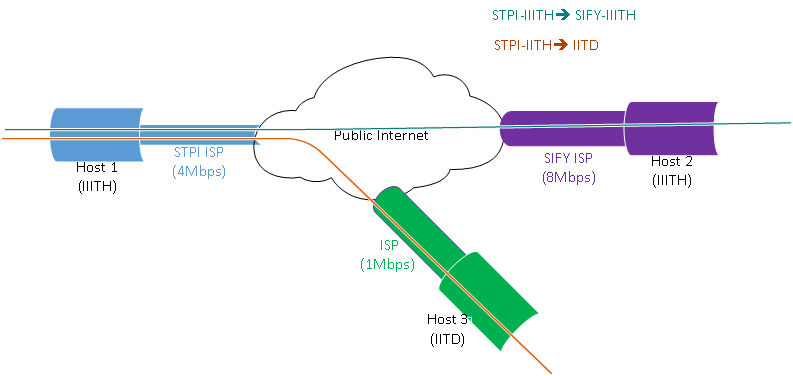
\includegraphics[width=16cm]{Performance Analysis Model.png}
\caption{Performance Analysis Model}
\end{figure}

\begin{itemize}
\item Following two models were used to test and estimate the link-speed:

\begin{itemize}
\item \textbf{STPI-IIITH to IITD}: Sample test-data was sent from one of the
      servers in IIITH on SIFY network to a test server located in IITD
\item \textbf{STPI-IIITH to SIFY-IIITH}: Sample test-data was sent from one
      of the servers at IIITH on SIFY network to another server on
      IIITH on STPI network
\end{itemize}

\end{itemize}
\begin{table}[H]
\caption{\label{tbl: Performance Modelling}Performance Modelling}
\begin{center}
\begin{tabular}{lllllll}
\hline
               &  Source  &  Destination  &  Average  &  Average   &  Average   &  Comments                \\
 Description   &  Upload  &  Download     &  Size     &  Duration  &  Achieved  &                          \\
               &  speed   &  speed        &  (GB)     &  (Hrs)     &  Speed     &                          \\
               &  (Mbps)  &  (Mbps)       &           &            &  (Mbps)    &                          \\
\hline
 STPI-IITH to  &  4       &  1            &  1.38     &  4.61      &  0.73      &                          \\
 IITD          &          &               &           &            &            &                          \\
\hline
 STPI-IITH to  &  4       &  8            &  1.38     &  0.64      &  4.93      &  - STPI more reliable    \\
 SIFY-IIITH    &          &               &           &            &            &  - Physical distance     \\
               &          &               &           &            &            &  matters                 \\
               &          &               &           &            &            &  - Achieved bandwidth    \\
               &          &               &           &            &            &  more because data gets  \\
               &          &               &           &            &            &  compressed              \\
\hline
\end{tabular}
\end{center}
\end{table}



\begin{table}[H]
\caption{\label{tbl: Performance Estimates}Performance Estimates}
\begin{center}
\begin{tabular}{lllll}
\hline
           &  Estimated  &  Source      &  Destination  &  Estimated  \\
           &  Average    &  Link-speed  &  Link-speed   &  Duration   \\
           &  Daily      &  upload      &  download     &  (Hrs)      \\
           &  Size(GB)   &  (Mbps)      &  (Mbps)       &             \\
\hline
 Phase-I   &  1.5        &  4           &  2            &  2.5        \\
 Phase-II  &  3          &  4           &  2            &  5          \\
\hline
\end{tabular}
\end{center}
\end{table}


\subsection{Reliability and Availability}
\label{sec-8.9}

\begin{itemize}
\item The solution is required to be available all the time (24*7*365).
\item Any outages at source or target mirror locations should be planned
   and notified apriori to that appropriate measures can be taken.
\item Following would be implemented at platform and network level:

\begin{itemize}
\item Hardware Level RAID Configuration would be used to ensure redundancy.
\item Multiple network ports on source and mirrored-system can be implemented.
\item Redundant power supply can ensure more availability.
\end{itemize}

\item No measures at the application level will be implemented to
   ensure further reliability and availability.
\end{itemize}
\subsection{Scalability}
\label{sec-8.10}

\begin{itemize}
\item The proposed solution is already planned to be scalable to the
     upper limits mentioned in the data characterstic specifications
     right from its inception and hence no specific
     scalability features would be implemented.
\end{itemize}
\section{OPERATIONS}
\label{sec-9}

\subsection{Monitoring}
\label{sec-9.1}

\begin{itemize}
\item The backup solution will be monitored manually once
   daily by the VLEAD Engineering team.
\end{itemize}
\subsection{Alarms and Notifications}
\label{sec-9.2}

\begin{itemize}
\item No automated alarms will configured. Will be tackled on a reactive
   basis as per the escalation matrix.
\item Email notifications will be configured to send the status or
   mirroring job everyday.
\end{itemize}
\subsection{Reporting}
\label{sec-9.3}

\begin{itemize}
\item No Reporting mechanisms are implemented as part of this solution.
\end{itemize}
\subsection{Capacity Planning}
\label{sec-9.4}

\begin{itemize}
\item Capacity planning for the entire solution is done in first stage
   itself and hence not required during operational phase of this
   project.
\end{itemize}
\section{SOLUTION ACCEPTANCE CRITERIA}
\label{sec-10}

 The solution should scalable for all the 180 labs and should be
   fast enough to run over-night and not affect normal operations of
   the systems and network.
\section{IMPLEMENTATION AND MIGRATION}
\label{sec-11}

 The solution is proposed to be implemented in two phases:


\begin{table}[H]
\caption{\label{tbl: Implementation Phases}Implementation Phases}
\begin{center}
\begin{tabular}{lll}
\hline
 Phase     &  Description                    &  Dependencies  \\
\hline
 Phase-I   &  Mirroring of Labs              &  None          \\
 Phase-II  &  Mirroring of VMs               &  Phase-I       \\
           &  and Disaster recovery testing  &                \\
\hline
\end{tabular}
\end{center}
\end{table}

 
 Detailed breakup and estimates of the subtasks can be found in
   ``D10-mirror-sources.org'' in VLEAD repository.
\subsection{Efforts and Schedule(Phase-I)}
\label{sec-11.1}



\begin{table}[H]
\caption{\label{tbl: Schedule and Estimates - PhaseI}Schedule and Estimates - PhaseI}
\begin{center}
\begin{tabular}{llll}
\hline
               &  Aug               &  Sep                    &  Oct                    \\
               &  2013              &  2013                   &  2013                   \\
\hline
 Deliverables  &  - Start Analysis  &  - Complete Analysis    &  -Develop and           \\
               &  - Tech-Specs      &  - Manual mirror setup  &  install pilot scripts  \\
               &                    &  at IITD                &  -Setup IITB mirror     \\
               &                    &                         &  manually               \\
\hline
 Effort        &  80Hrs             &  80Hrs                  &  80Hrs                  \\
 Estimates     &                    &                         &                         \\
\hline
\end{tabular}
\end{center}
\end{table}



\begin{center}
\begin{tabular}{llllll}
\hline
               &  Nov                     &  Dec   &  Jan   &  Feb   &  Mar   \\
               &  2013                    &  2013  &  2013  &  2013  &  2013  \\
\hline
 Deliverables  &  - Deploy final scripts  &  X     &  X     &  X     &  X     \\
               &  - Test and Fix issues   &        &        &        &        \\
               &  - Documentation         &        &        &        &        \\
\hline
 Effort        &  80hrs                   &  X     &  X     &  X     &  X     \\
 Estimates     &                          &        &        &        &        \\
\hline
\end{tabular}
\end{center}



\subsection{Efforts and Schedule(Phase-II)}
\label{sec-11.2}




\begin{center}
\begin{tabular}{ll}
\hline
               &  Schedule         \\
\hline
 Deliverables  &  Not yet planned  \\
\hline
 Effort        &  180 hrs          \\
 Estimates     &                   \\
\hline
\end{tabular}
\end{center}



\subsection{Migration Requirements}
\label{sec-11.3}

   Since, the solution is built from scratch, no specific migration requirements
   are to be addressed
\section{REFERENCES}
\label{sec-12}



\begin{table}[H]
\caption{\label{tbl: References}References}
\begin{center}
\begin{tabular}{lll}
\hline
 Document  &  Title                    &  Location                   \\
 Number    &                           &                             \\
\hline
           &  VLEAD Expert Committee   &  <Vlead-Repo>               \\
           &  Review - 25 July 2013    &  /meetings-and-reviews      \\
           &  Presentation             &  /2013-07-25-expert-review  \\
           &                           &  /src/index.org             \\
           &  VLEAD Engg Contract      &  <Vlead-Repo>               \\
           &                           &  /official-docs             \\
           &                           &  /2012-06-02-vlead-         \\
           &                           &  engg-contract.pdf          \\
           &  Mirroring to IITD -      &                             \\
           &  Sub-tasks and Estimates  &  <Vlead-Repo>               \\
           &                           &  /plans//project-plan       \\
           &                           &  /grand-prix/estimates      \\
           &                           &  /D10-mirror-sources.org    \\
\hline
\end{tabular}
\end{center}
\end{table}


\section{DEFINITIONS}
\label{sec-13}

The following words, acronyms and abbreviations are referred to in
this document.


\begin{table}[H]
\caption{\label{tbl: Definitions}Definitions}
\begin{center}
\begin{tabular}{ll}
\hline
 Term        &  Definition                                              \\
\hline
 VLEAD       &  Virtual Labs Engineering and Architecture Divison       \\
 RAID        &  Redundant Array of Independent Disks                    \\
 Engg        &  Engineering                                             \\
 IITD        &  Indian Institute of Technology, Delhi                   \\
 IIIT        &  International Institute of Information Technology       \\
 VM          &  Virtual Machines                                        \\
 Containers  &  Light-weight Virtual machines                           \\
 SAN         &  Storage Area Network                                    \\
 SSH         &  Secure Shell                                            \\
 HTTP        &  HyperText Transfer (or Transport) Protocol,             \\
             &  the data transfer protocol used on the World Wide Web.  \\
\hline
\end{tabular}
\end{center}
\end{table}

\section{ATTACHMENTS}
\label{sec-14}



\begin{center}
\begin{tabular}{ll}
\hline
 Document Number  &  Title  \\
\hline
\end{tabular}
\end{center}



\section{SIGN-OFF}
\label{sec-15}

The completion of the sign-off page is a testament by the signatories
below that the following has been achieved or agreed:
\begin{itemize}
\item The document has been peer reviewed and all review-defects have been fixed
\item The document is complete and accurate
\item This document will be placed under configuration control
\end{itemize}
\begin{table}[H]
\caption{\label{tbl: Sign-Off}Sign-Off}
\begin{center}
\begin{tabular}{lr}
\hline
 Reviewed Revision Number  &                0.2  \\
 Baseline Revision Number  &                     \\
 Baseline Date             &                     \\
 Author                    &  Suraj Ketan Samal  \\
\hline
\end{tabular}
\end{center}
\end{table}

                        


\begin{center}
\begin{tabular}{lll}
\hline
 Name                     &  Ranjan Bose                       &  Contact Number  \\
                          &                                    &  +91-11-2659104  \\
 Organizational Position  &  Professor,                        &                  \\
                          &  Dept. of Electrical Engineering,  &                  \\
                          &  IIT Delhi                         &                  \\
 Signature                &  <Attach e-mail approval           &  Date            \\
                          &  or link to approval>              &                  \\
 Role                     &  Project Co-Investigator,          &                  \\
                          &  Virtual Labs Project              &                  \\
\hline
\end{tabular}
\end{center}




\begin{center}
\begin{tabular}{lll}
\hline
 Name                     &  Venkatesh Choppella      &  Contact Number    \\
                          &                           &  +91-965-274-0281  \\
 Organizational Position  &  Associate Professor,     &                    \\
                          &  IIIT Hyderabad           &                    \\
 Signature                &  <Attach e-mail approval  &  Date              \\
                          &  or link to approval>     &                    \\
 Role                     &  Head, VLEAD Project      &                    \\
\hline
\end{tabular}
\end{center}



\subsection{Major Comments}
\label{sec-15.1}

   
\subsection{Documentation Location}
\label{sec-15.2}


\begin{center}
\begin{tabular}{ll}
\hline
 Master Hard copy  &  Master Electronic                                  \\
\hline
 None              &  Stored in `mirror' bzr repository on VLEAD server  \\
\hline
\end{tabular}
\end{center}


  
\section{DOCUMENT CONTROL SHEET}
\label{sec-16}

This section captures all changes made to the content of document. If
you have any questions regarding this document or would like to
suggest an improvement, contact:



\begin{table}[H]
\caption{\label{tbl: Contact for Enquiries}Contact for Enquiries}
\begin{center}
\begin{tabular}{ll}
\hline
 Name         &  Suraj Ketan Samal        \\
 Designation  &  Project Engineer         \\
 Phone        &  +91 40 6653 1592         \\
 Email        &  engg@virtual-labs.ac.in  \\
 Fax          &  <Contact Fax>            \\
\hline
\end{tabular}
\end{center}
\end{table}




\begin{table}[H]
\caption{\label{tbl: Record of Issues}Record of Issues}
\begin{center}
\begin{tabular}{rrll}
\hline
 Issue No  &  Issue Date  &  Nature of Amendment    &  Author  \\
\hline
      0.1  &  2013-08-21  &  Initial Draft          &  Suraj   \\
      0.2  &  2013-09-05  &  Updated with analysis  &  Suraj   \\
           &              &  and estimates          &          \\
\hline
\end{tabular}
\end{center}
\end{table}


This publication has been prepared and written by \textbf{VLEAD,IIIT Hyderabad}, and is copyright. Other than for the purposes of and
subject to the conditions prescribed under the Copyright Act, no part
of it may in any form or by any means (electronic, mechanical,
microcopying, photocopying, recording or otherwise) be reproduced,
stored in a retrieval system or transmitted without prior written
permission from the document controller.

Note for other readers: The contents of this publication are subject
to change without notice. All efforts have been made to ensure the
accuracy of this publication. Notwithstanding, \textbf{VLEAD, IIIT Hyderabad}
does not assume responsibility for any errors nor for any consequences
arising from any errors in this publication.

\end{document}
